\documentclass[aspectratio=169,10pt]{beamer}
\usepackage{fontspec}
\usepackage[polish]{babel}
\setmonofont{NotoSansMono-Regular.ttf}[Scale=0.85]
\usepackage{booktabs,graphicx,fvextra}
\newcommand{\autor}{Damian Osiński}
\newcommand{\album}{[nr albumu]}
\newcommand{\uczelnia}{[uczelnia, wydział, kierunek]}
\newcommand{\prowadzacy}{[prowadzący]}
\newcommand{\datapracy}{listopad 2026}

\graphicspath{{img/}}
\usetheme{default}
\usefonttheme{professionalfonts}
\definecolor{v}{HTML}{B3261E}
\definecolor{s}{HTML}{1B6E3C}
\definecolor{k}{HTML}{1F3A5F}
\setbeamercolor{frametitle}{fg=k}\setbeamercolor{title}{fg=k}\setbeamercolor{structure}{fg=k}
\setbeamerfont{frametitle}{series=\bfseries,size=\Large}
\setbeamertemplate{navigation symbols}{}
\setbeamertemplate{footline}{\hfill\scriptsize\insertframenumber/\inserttotalframenumber\hspace{4mm}\vspace{2mm}}
\newcommand{\kod}[1]{\texttt{#1}}
\newcommand{\vuln}{\textcolor{v}{\textbf{VULN}}}
\newcommand{\secure}{\textcolor{s}{\textbf{SECURE}}}
\title{Aplikacja CRUD w~wersji zabezpieczonej i~niezabezpieczonej}
\subtitle{Analiza zachowania i~ruchu sieciowego}
\author{\autorzy\\grupa \grupa}
\institute{\przedmiot\\\uczelnia}
\date{\today}
\begin{document}

\begin{frame}[plain]\titlepage\end{frame}

\begin{frame}{Jeden kod, dwa tryby}
\begin{columns}[T]
\column{.5\textwidth}
\textbf{notes-cyber-project}: notatnik wieloużytkownikowy, pełny CRUD\\[2mm]
\begin{itemize}
\item \vuln: HTTP :3000, zabezpieczenia wyłączone
\item \secure: HTTPS :3443, zabezpieczenia włączone
\item przełącza je jedna zmienna \kod{SECURE}
\item Node.js, Express, SQLite w~pamięci
\end{itemize}
\vspace{2mm}
Różnice w~wynikach wynikają tylko z~zabezpieczeń.
\column{.42\textwidth}
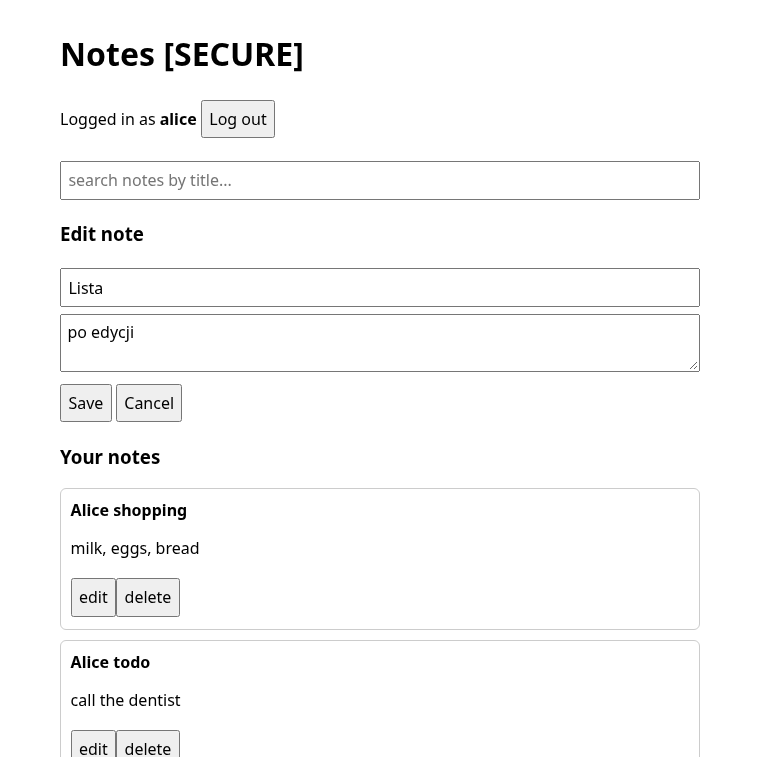
\includegraphics[height=.75\textheight]{secure-edit}
\end{columns}
\end{frame}

\begin{frame}{Dobór technik}\footnotesize
\begin{tabular}{lll}
\toprule
Problem & Wybór & Dlaczego\\\midrule
SQL injection & zapytania parametryzowane & usuwają klasę błędu, zamiast filtrować\\
XSS & \kod{textContent} + CSP & dwie niezależne warstwy\\
Hasła & scrypt $2^{14}/8/5$ & \kod{node:crypto}, parametry z~listy OWASP\\
Sesja & losowe 256 b, cookie \kod{\_\_Host-} & unieważnialna, niedostępna dla JS\\
CSRF & token + \kod{SameSite=Strict} & samo cookie nie wystarcza\\
Brute force & 5 nieudanych prób / 60 s & bez blokowania konta ofiary\\
Transmisja & TLS 1.3 & poufność i~integralność\\
\bottomrule
\end{tabular}
\end{frame}

\begin{frame}{\vuln: hasło widać w~jednym pakiecie}
\centering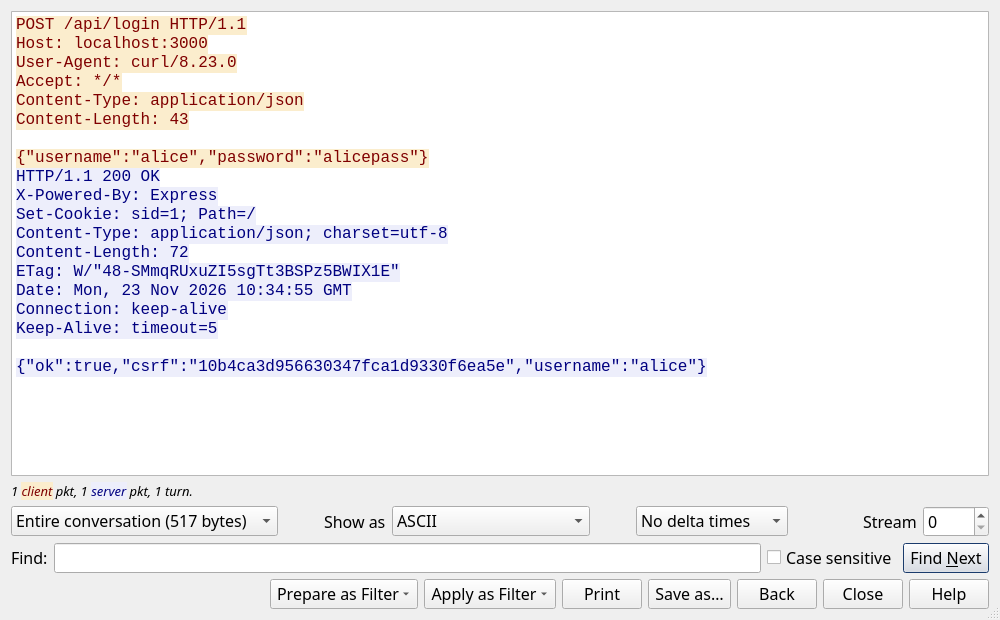
\includegraphics[height=.78\textheight]{ws-vuln-follow}
\end{frame}

\begin{frame}{\secure: to samo logowanie}
\centering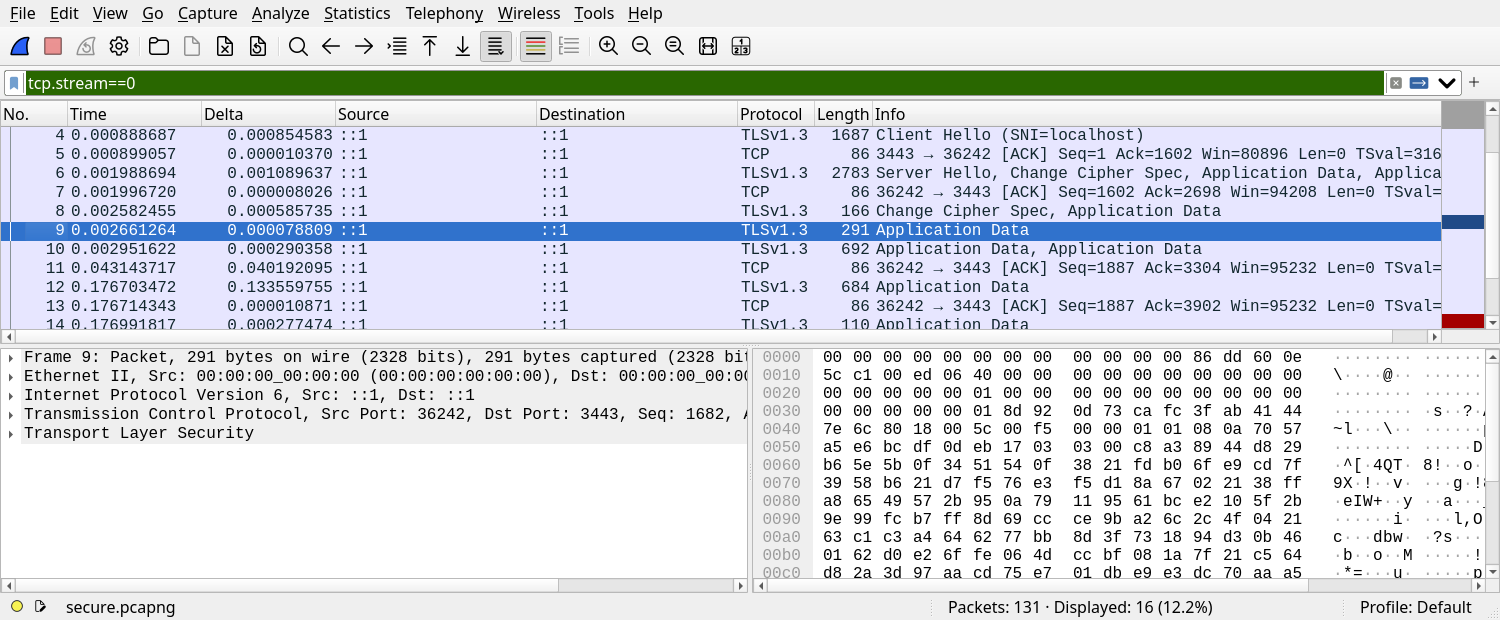
\includegraphics[width=.95\linewidth]{ws-secure-list}
\end{frame}

\begin{frame}{Co znajdzie podsłuchujący?}
\begin{columns}[T]
\column{.5\textwidth}
\begin{tabular}{lrr}
\toprule
Ramki z~ciągiem & \vuln & \secure\\\midrule
hasło & 1 & 0\\
treść notatki & 4 & 0\\
\kod{csrf} & 2 & 0\\
\kod{Cookie} & 8 & 0\\
adresy \kod{/api/notes} & 6 & 0\\
nazwa serwera (SNI) & 8 & 8\\
\bottomrule
\end{tabular}
\column{.45\textwidth}
\begin{itemize}
\item \vuln: cookie z~przechwyconego pliku wystarczyło do przejęcia sesji
\item \secure: TLS 1.3, AES-256-GCM, X25519MLKEM768 (hybryda odporna kwantowo)
\end{itemize}
\end{columns}
\end{frame}

\begin{frame}{TLS nie ukrywa rozmiarów ani czasu}
\begin{columns}[T]
\column{.45\textwidth}
\small
\begin{tabular}{lrr}
\toprule
Operacja & HTTP [B] & TLS [B]\\\midrule
logowanie & 183 & 200\\
lista & 204 & 221\\
utworzenie & 317 & 334\\
odczyt & 206 & 223\\
edycja & 318 & 335\\
wyszukiwanie & 212 & 229\\
usunięcie & 257 & 274\\
sesja & 201 & 218\\
\bottomrule
\end{tabular}
\column{.5\textwidth}
\begin{itemize}
\item rekord = dane + \textbf{17 B}, zawsze
\item osiem operacji, osiem różnych długości
\item logowanie zdradza też czas: ok. 174 ms (scrypt)
\item kanał boczny: Chen i~in., IEEE S\&P 2010
\end{itemize}
\end{columns}
\end{frame}

\begin{frame}{Koszt zabezpieczeń}
\begin{tabular}{lrr}
\toprule
& \vuln & \secure\\\midrule
bajty, 8 operacji, nowe połączenia & 10\,706 & 57\,197\\
nowe połączenie & 0{,}57 ms & 2{,}79 ms\\
to samo połączenie & 0{,}13 ms & 0{,}14 ms\\
logowanie & 0{,}86 ms & 172{,}69 ms\\
\bottomrule
\end{tabular}
\begin{itemize}
\item koszt TLS to uzgodnienie; przy keep-alive jest pomijalny
\item wolne logowanie jest celowe: tyle płaci napastnik za każde hasło
\end{itemize}
\end{frame}

\begin{frame}{11 podatności}
\footnotesize
\begin{tabular}{rllll}
\toprule
& Podatność & OWASP 2025 & \vuln & \secure\\\midrule
1 & Brak szyfrowania & A04 & hasło czytelne & 0 ramek\\
2 & SQL injection & A05 & zrzut kont & 401, pusta lista\\
3 & Trwały XSS & A05 & skrypt działa & zwykły tekst\\
4 & Hasła jawne & A04 & \kod{alicepass} & skrót scrypt\\
5 & IDOR & A01 & cudza notatka & 404\\
6 & Atrybuty cookie & A02 & brak & komplet\\
7 & CSRF & A01 & notatka utworzona & 401 / 403\\
8 & Brak limitu logowań & A07 & hasło znalezione & 429\\
9 & Brak nagłówków & A02 & brak & CSP, HSTS\dots\\
10 & Przewidywalna sesja & A07 & \kod{sid=1} & 401\\
11 & Ślad stosu & A10 & ścieżki plików & komunikat ogólny\\
\bottomrule
\end{tabular}
\end{frame}

\begin{frame}[fragile]{Łańcuch: SQL injection i~jawne hasła}
\textcolor{v}{\textbf{VULN}}
\begin{Verbatim}[fontsize=\footnotesize,breaklines]
q = x%' UNION SELECT id, username, password FROM users --
[{"id":1,"title":"alice","body":"alicepass"},{"id":2,"title":"bob","body":"bobsecret"}]
\end{Verbatim}
\textcolor{s}{\textbf{SECURE}}
\begin{Verbatim}[fontsize=\footnotesize]
[]
\end{Verbatim}
Przy skrótach scrypt nawet udany zrzut nie dałby gotowych haseł.
\end{frame}

\begin{frame}{Trwały XSS}
\begin{columns}[T]
\column{.48\textwidth}\centering\vuln\\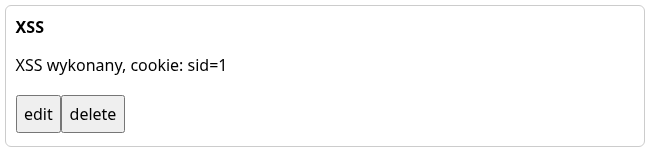
\includegraphics[width=\linewidth]{vuln-xss}
\column{.48\textwidth}\centering\secure\\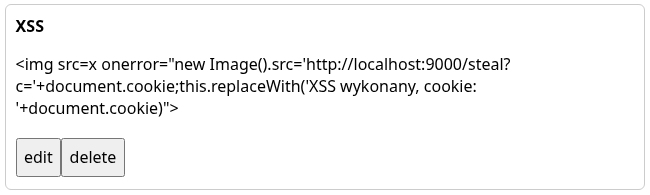
\includegraphics[width=\linewidth]{secure-xss}
\end{columns}
\end{frame}

\begin{frame}{CSRF: przeglądarki się różnią}
\small
\begin{tabular}{lll}
\toprule
Scenariusz & Chrome 158 & Firefox 160\\\midrule
\vuln, inna witryna, świeże cookie & udany & udany\\
\vuln, inna witryna, cookie sprzed 130 s & zablokowany & udany\\
\secure, \kod{127.0.0.1:9000} & 401 & 401\\
\secure, \kod{http://localhost:9000} & 401 & \textbf{403}\\
\bottomrule
\end{tabular}
\begin{itemize}
\item Firefox wysłał cookie \kod{SameSite=Strict}, bo pomija schemat przy porównaniu witryn
\item atak zatrzymał dopiero token CSRF: obrona warstwowa
\item \kod{fetch} z~\kod{DELETE} nie działa (preflight CORS), formularz POST tak
\end{itemize}
\end{frame}

\begin{frame}{Weryfikacja i~ograniczenia}
\begin{columns}[T]
\column{.47\textwidth}
\textbf{Weryfikacja}
\begin{itemize}
\item \kod{npm test}: 28 testów, oba tryby
\item usunięcie dowolnego z~6 sprawdzonych zabezpieczeń wykryte
\item \kod{report/collect.sh} odtwarza pomiary
\end{itemize}
\column{.47\textwidth}
\textbf{Dalszy rozwój}
\begin{itemize}
\item hasła $\geq$ 15 znaków (NIST), Argon2id, passkeys
\item limit logowań na konto
\item dziennik zdarzeń bezpieczeństwa
\item ECH, dopełnianie rekordów TLS
\item CI: testy, \kod{npm audit}, ZAP
\end{itemize}
\end{columns}
\end{frame}

\begin{frame}{Wnioski}
\begin{enumerate}
\item HTTP: podsłuch jednego połączenia daje hasło i~sesję.
\item TLS chroni treść, ale nie rozmiary i~czasy.
\item TLS nie naprawia błędów aplikacji (SQLi, IDOR, XSS).
\item Pojedyncze zabezpieczenie bywa zawodne, potrzebne są warstwy.
\end{enumerate}
\vspace{5mm}
\textbf{Pokaz na żywo:} \kod{npm run start:vuln}, \kod{npm run start:secure}, \kod{attacks/}
\end{frame}
\end{document}
